\documentclass[a4paper,12pt,oneside,openany,brazil]{abntex2}

\usepackage[T1]{fontenc}
\usepackage[utf8]{inputenc}
\usepackage[brazil]{babel}
\usepackage{geometry}
\usepackage{lmodern}
\usepackage{amsmath}
\usepackage{amssymb}
\usepackage{setspace}
\usepackage{xr-hyper}
\usepackage{hyperref}
\usepackage{xcolor}
\usepackage{graphicx}
\usepackage{placeins}
\usepackage[alf,no-abnt-option-file]{abntex2cite}
% Configuração local das citações; referências restritas às obras citadas.
\citeoption{config-citacoes-abnt}

\geometry{
    top=3cm,
    bottom=2cm,
    left=3cm,
    right=2cm
}

\setlength{\parindent}{1.25cm}
\setlength{\parskip}{0pt}
\OnehalfSpacing
\raggedbottom

% Citações indiretas: \cite{chave} ou \citeonline{chave}.
% Citações diretas curtas: ``trecho'' com \cite[p.~45]{chave},
% ou \citeonline[p.~45]{chave} antes do trecho entre aspas.
% Citações diretas com mais de três linhas: ambiente citacao, sem aspas,
% com autoria, ano e página. O espaço externo acompanha uma linha do corpo.
\setlength{\ABNTEXcitacaorecuo}{4cm}
\newlength{\espacocitacao}
\setlength{\espacocitacao}{\baselineskip}
\renewenvironment{citacao}{%
    \par\addvspace{\espacocitacao}%
    \begin{list}{}{%
        \setlength{\leftmargin}{\ABNTEXcitacaorecuo}%
        \setlength{\rightmargin}{0pt}%
        \setlength{\listparindent}{0pt}%
        \setlength{\itemindent}{0pt}%
        \setlength{\topsep}{0pt}%
        \setlength{\partopsep}{0pt}%
        \setlength{\parsep}{0pt}%
        \setlength{\itemsep}{0pt}%
    }%
    \item\relax
    \SingleSpacing\fontsize{10}{12}\selectfont
}{%
    \end{list}%
    \par\addvspace{\espacocitacao}%
}

% Numeração das seções sem o prefixo do capítulo
\renewcommand{\thesection}{\arabic{section}}
\renewcommand{\thesubsection}{\arabic{section}.\arabic{subsection}}
\renewcommand{\thesubsubsection}{\arabic{section}.\arabic{subsection}.\arabic{subsubsection}}
% O ponto pertence ao título da seção, não ao número recuperado por \ref.
\setsecnumformat{\csname the#1\endcsname\ifstrequal{#1}{section}{.}{}\quad}


\hypersetup{colorlinks=true,linkcolor=black,citecolor=black,urlcolor=black}
\renewcommand{\figurename}{Figura}

\externaldocument[S-]{supplementary_material_JEM}[supplementary_material_JEM.pdf]
\begin{document}
\pagestyle{plain}
\aliaspagestyle{chapter}{plain}
\begin{center}
{\Large\bfseries Preços agrícolas, capacidade produtiva e perdas anteriores na conversão da vegetação nativa em Mato Grosso}\\[0.5cm]
Fernando Souza da Vieira
\end{center}

\noindent\textbf{Resumo}

A expansão agropecuária pode ocorrer pelo aproveitamento de áreas abertas ou pela conversão da vegetação, com implicações distintas para a gestão ambiental. Este artigo examina como preços reais de soja e milho se associam à conversão bruta para agricultura em Mato Grosso e como essa associação varia com a capacidade produtiva potencial e as perdas anteriores. O painel municipal de 2001--2024 combina MapBiomas, PAM, GAEZ, preços internacionais e clima, com efeitos fixos municipais e de bioma por ano. A associação preço×capacidade diminui quando se exige o histórico necessário às perdas. Para +10\% no preço e dez pontos percentuais adicionais de perda, os contrastes são 0,0040 p.p. na soja e $-0,0001$ p.p. no milho, com intervalos de 95\% abrangendo zero nas três inferências. Comparações com pastagem e entre períodos revelam heterogeneidade sensível à amostra e à inferência. As exposições geográficas utilizadas não identificam efeitos do Código Florestal ou da Moratória da Soja. Os resultados indicam a necessidade de distinguir destinos, condições produtivas e cobertura dos dados ao interpretar pressões sobre a vegetação, sem deduzir ausência de resposta aos preços ou mecanismos financeiros da imprecisão dos contrastes.

\medskip
\noindent\textbf{Palavras-chave:} conversão da vegetação; preços agrícolas; capacidade produtiva; quebras de safra; gestão ambiental.

\medskip
\noindent\textbf{Destaques}
\begin{itemize}
\item Produção e conversão da vegetação descrevem margens distintas de expansão.
\item O histórico produtivo altera a amostra e os gradientes estimados.
\item Os contrastes de perdas são imprecisos no núcleo de soja e milho.
\item Exposição territorial não mede cumprimento ou efeito das políticas.
\end{itemize}

\section{Introdução}
\label{sec:introducao}
%%% REF5--REF12: síntese editorial; preservam-se pergunta e hipóteses do original.

A expansão agropecuária envolve escolhas que têm consequências distintas para a vegetação nativa. Produzir mais pode exigir novas áreas, mas também pode resultar de maior rendimento, de uma segunda safra ou da substituição de um uso já estabelecido. Para a gestão ambiental, essa diferença impede que o crescimento da oferta seja tomado, por si só, como medida da pressão de abertura. Em Mato Grosso, a expansão da produção de soja e milho coexistiu com taxas de conversão menores nos extremos de 2001--2024, enquanto a pastagem predominou entre os destinos das áreas abertas na amostra ambiental fixa. O interesse dessa coexistência está em compreender como os incentivos econômicos se associam à conversão diante de possibilidades produtivas e restrições que variam entre territórios.

Sob a ótica econômica, a escolha entre conservar e converter depende dos benefícios e custos das alternativas acessíveis ao produtor. A receita agrícola é apropriável, enquanto parte dos serviços mantidos pela vegetação beneficia outros agentes, de modo que a alternativa privada mais atraente pode divergir daquela que considera as perdas ambientais \cite{Angelsen2010}. O custo de oportunidade da conservação corresponde ao benefício líquido da melhor alternativa a que se renuncia, e não apenas ao valor da produção que poderia ocupar a área. Essa comparação reúne condições agronômicas, custos de abertura e produção, acesso a mercados e restrições institucionais. A participação do ambiente no processo econômico aparece tanto nas possibilidades de produzir quanto nos serviços perdidos com a conversão.

Os preços participam dessa escolha sem determinar uma resposta territorial uniforme. Mantidos os custos e as demais condições, uma alta da cotação representa maior acréscimo de receita por hectare onde a produção potencial da cultura é maior. Essa vantagem pode favorecer o aproveitamento de áreas abertas ou tornar mais atraente a expansão sobre vegetação. \citeonline{LubowskiEtAl2008} relacionaram decisões de uso da terra a retornos líquidos e qualidade da terra nos Estados Unidos, enquanto \citeonline{Pfaff1999} destacou características locais e custos de transporte na Amazônia. Em escala tropical, \citeonline{BermanEtAl2023} combinaram preços internacionais e aptidão agrícola e encontraram associação positiva com desmatamento, heterogênea conforme as condições econômicas. Esses estudos justificam examinar a exposição diferencial a preços comuns, sem transferir automaticamente suas magnitudes ou condições de identificação para Mato Grosso.

Também importa distinguir o uso que cresce daquele que cede espaço. Na bacia do Tapajós, \citeonline{Braganca2018} encontrou que a valorização das lavouras em relação à carne favoreceu a substituição de pastagens por cultivos e reduziu o desmatamento local, sob condições próprias de realocação de fatores. Na porção florestal de Mato Grosso, \citeonline{MacedoEtAl2012} observaram que a expansão da soja entre 2006 e 2010 ocorreu principalmente em terras já abertas, enquanto novas pastagens responderam pela maior parte do desmatamento remanescente. Portanto, a conversão diretamente para agricultura não esgota a relação entre valorização dos grãos e transformação territorial. A comparação com pastagens amplia a leitura dos destinos, embora não permita localizar deslocamentos indiretos ou identificar a cultura que motivou cada abertura.

A capacidade potencial, por sua vez, não descreve todas as condições em que uma localidade responde aos preços. O desempenho das safras anteriores pode alterar recursos e alternativas de investimento. Uma perda produtiva pode restringir a capacidade de aproveitar uma valorização, mas também pode ser seguida de expansão quando houver terra e financiamento disponíveis. A evidência sobre crédito e risco oferece razões para considerar essas possibilidades. Na Amazônia brasileira, \citeonline{AssuncaoEtAl2020Credito} estimaram redução do desmatamento após o condicionamento ambiental do crédito, com efeito mais evidente em municípios voltados à pecuária e estimativa imprecisa nos voltados às lavouras. Em Gana, \citeonline{KarlanEtAl2014} encontraram aumento do investimento agrícola com seguro, distinguindo risco não segurado de falta de capital. Nenhum desses resultados demonstra que uma quebra de soja ou milho em Mato Grosso reduza recursos e, por essa via, a conversão posterior.

Perdas produtivas também foram acompanhadas de outras respostas territoriais. Na Zâmbia, \citeonline{OrdonezEtAl2025} examinaram uma infestação de lagarta-do-cartucho e encontraram perdas, aumento da produção de carvão e expansão de lavouras. A expansão foi imprecisa no painel de famílias e apareceu na análise espacial, distinção que impede reunir extração e abertura numa única resposta. Em texto para discussão, \citeonline{HsiaoEtAl2026} relacionaram calor extremo, perda florestal e expansão de lavouras; para o Brasil, encontraram redução da produtividade física acompanhada de aumento dos preços agrícolas locais. Os estudos mostram que perda física, receita e expansão podem seguir trajetórias diferentes, mas não estabelecem uma intenção compensatória comum aos produtores nem reproduzem o contraste municipal com cotações internacionais aqui investigado.

As instituições condicionam essas alternativas ao modificar o acesso a recursos e mercados e os custos do descumprimento. A existência da regra não equivale à sua implementação \cite{North1991}. \citeonline{HeilmayrEtAl2020} estimaram redução do desmatamento em áreas aptas à soja no bioma Amazônia após a Moratória, enquanto \citeonline{HardingEtAl2021} examinaram diferenças na resposta aos preços sob instrumentos de conservação. Efeito médio de uma política e alteração da sensibilidade aos incentivos são perguntas distintas. O Código Florestal estabelece obrigações por imóvel; a Moratória condiciona a comercialização da soja segundo critérios do acordo. Por isso, bioma, cobertura florestal e autuações não podem ser tratados como medidas equivalentes de exposição ou cumprimento.

O problema de pesquisa consiste em compreender como os preços agrícolas se associam à taxa de conversão bruta da vegetação nativa para agricultura em Mato Grosso e de que maneira essa associação varia com a capacidade produtiva local e as quebras de safra anteriores, considerando os biomas e a exposição ao Código Florestal e à Moratória da Soja. Soja e milho são as culturas centrais, e a pastagem participa como destino complementar. O preço da carne contextualiza incentivos entre atividades. Valorização patrimonial e apropriação irregular da terra permanecem fora do objeto empírico.

\noindent\textbf{H1 --- Preços, perdas produtivas e conversão da vegetação.} A associação entre os preços reais de soja e milho e a taxa de conversão bruta da vegetação nativa para agricultura depende da capacidade produtiva potencial local e é modificada por quebras de safra anteriores.

\noindent\textbf{H1a --- Preços e capacidade produtiva potencial.} Essa associação é mais positiva nos municípios com maior capacidade produtiva potencial da respectiva cultura, mantidas as demais condições relevantes.

\noindent\textbf{H1b --- Quebras de safra e resposta aos preços.} A ocorrência e a intensidade de quebras de safra anteriores modificam a associação entre preços reais e conversão bruta subsequente, mantidas as demais condições relevantes. Não se determina previamente o sinal dessa modificação.

O artigo articula potencial agronômico, desempenho realizado e conversão por destino numa base municipal integrada, separando mudança de composição amostral de mudança de especificação. A dimensão temporal ordena perda, preço e conversão, sem demonstrar expectativas ou planejamento individual. Na dimensão institucional, a ausência de obrigações e passivos históricos validados por imóvel restringe a comparação do Código à heterogeneidade pela cobertura florestal inicial em torno da reforma de 2012. Para a Moratória, utiliza-se alcance territorial potencial. Essas medidas delimitam a parte da pergunta que o desenho pode examinar, sem identificar efeitos das políticas.

Os resultados mostram que os gradientes preço×capacidade diminuem quando se exige o histórico necessário às perdas, antes mesmo de acrescentar seus termos. No núcleo, os intervalos dos gradientes de H1a e dos modificadores de H1b abrangem zero. Comparações por período, destino e exposição territorial revelam heterogeneidade dependente do suporte e da inferência. A contribuição para a gestão ambiental está em distinguir o que essas informações permitem reconhecer e o que permanece incerto, evitando deduzir abertura do crescimento produtivo ou eficácia institucional de uma diferença de coeficientes. A apresentação segue das condições locais e da construção das medidas aos contrastes, reservando à discussão suas implicações e limites; o desenvolvimento conceitual ampliado encontra-se no Texto~\ref{S-text:s1} do suplemento.

\section{Área de estudo e dados}
\label{sec:dados}

Mato Grosso reúne Amazônia, Cerrado e Pantanal, com diferenças ambientais e trajetórias de ocupação que participam das possibilidades agrícolas. A análise utiliza os 141 municípios da malha IBGE de 2023 entre 2001 e 2024. Boa Esperança do Norte não constitui unidade autônoma nessa grade. O bioma de maior fração municipal organiza a comparação territorial, preservando-se as frações dos demais biomas. Há 63 municípios mistos, e a classificação predominante não localiza cada conversão dentro de um bioma nem representa regra uniforme para todos os imóveis. O mapa e a cobertura territorial detalhada estão na Figura~\ref{S-fig:h1-uso-solo} e na Tabela~\ref{S-tab:h1-cobertura}.

A produção e as áreas plantada e colhida provêm da Produção Agrícola Municipal (PAM), e as transições anuais de uso da terra, do MapBiomas Coleção 10.1 \cite{IBGEPAM2026,MapBiomas2026}. A grade contém 3.384 pares município--ano potenciais, dos quais 2.772, em 137 municípios, têm cobertura completa das transições. Os 612 restantes não são tratados como conversões observadas, mesmo quando a base auxiliar contém valores preenchidos. A comparabilidade exige ainda distinguir essa cobertura ambiental da continuidade do cultivo e do histórico usado para medir perdas.

A Figura~\ref{fig:h1-conversao} confronta os dois destinos imediatos da abertura. Em cada ano, soma-se a vegetação convertida e divide-se pelo estoque nativo inicial dos mesmos municípios, em porcentagem. A linha azul acompanha os 95 municípios com informação nos 24 anos; a cinza tracejada reúne os disponíveis no ano. Trata-se de razão de somas, diferente da média das taxas municipais utilizada em outras comparações. Nos extremos do período, as taxas de ambos os destinos foram menores em 2024 que em 2001, e a pastagem permaneceu acima da agricultura na amostra fixa. Essa coexistência com a expansão dos grãos situa a distinção entre produzir mais, reorganizar áreas abertas e converter vegetação.

\begin{figure}[htbp]
\centering
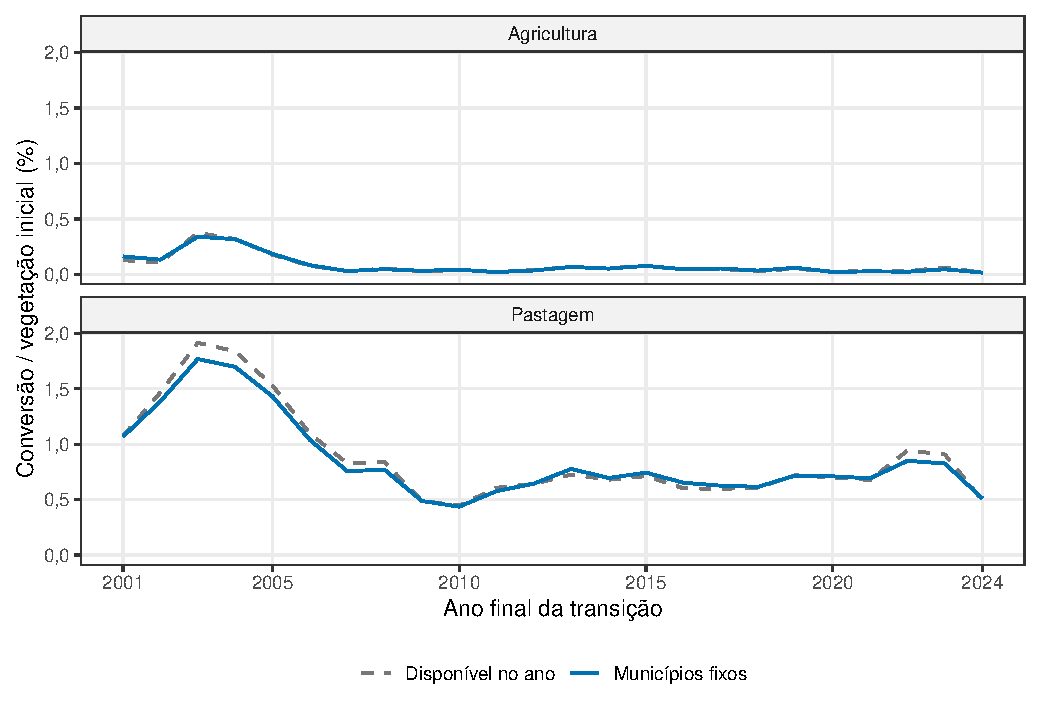
\includegraphics[width=\textwidth]{assets/fig01_conversao.pdf}
\caption{Conversão bruta da vegetação nativa para agricultura e pastagem, 2001--2024}
\label{fig:h1-conversao}
\begin{minipage}{\textwidth}\footnotesize\centering
Fonte: elaboração própria com MapBiomas 10.1 e malha IBGE 2023.
\end{minipage}
\end{figure}
\FloatBarrier

Os preços internacionais de soja, milho e carne bovina provêm da \textit{Pink Sheet}. As cotações mensais foram deflacionadas pelo CPI-U para dólares de poder de compra médio de 2024, exigindo doze meses para cada média anual \cite{WorldBank2026,BLSCPI2026}. A Figura~\ref{fig:h1-precos} apresenta índices com base 100 em 2000, permitindo comparar variações proporcionais entre produtos cotados em unidades diferentes. Os preços de 2000--2023 antecedem as conversões de 2001--2024. Em 2023, as três cotações reais superavam as de 2000, embora as taxas de conversão fossem menores nos extremos correspondentes. Essa comparação descritiva reúne mudanças de contexto e não identifica a resposta condicionada aos preços.

\begin{figure}[htbp]
\centering
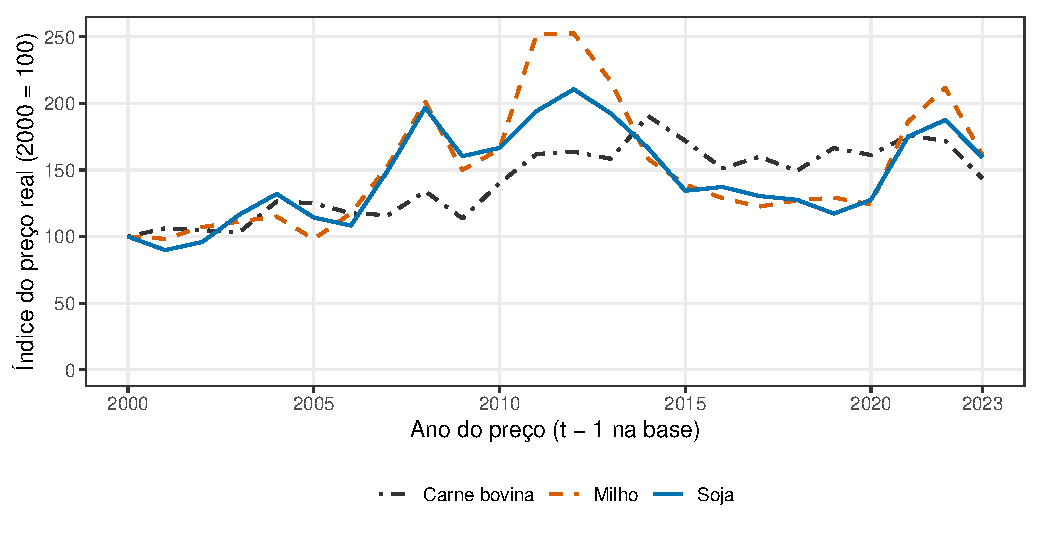
\includegraphics[width=\textwidth]{assets/fig03_precos.pdf}
\caption{Preços reais internacionais de soja, milho e carne bovina}
\label{fig:h1-precos}
\begin{minipage}{\textwidth}\footnotesize\centering
Fonte: elaboração própria com Banco Mundial e CPI-U BLS/FRED.
\end{minipage}
\end{figure}
\FloatBarrier

O potencial agrícola é medido pelo GAEZ v4 em sequeiro e alto insumo, em quilogramas de matéria seca por hectare \cite{FAOGAEZ2021}. O indicador da melhor classe de aptidão de cada célula foi agregado por média dos pixels válidos, ponderada pelo cosseno da latitude para aproximar suas áreas. A climatologia é 1961--1990, mas a versão incorpora bases territoriais de 2010. Portanto, o indicador fixo não garante anterioridade de todos os componentes às decisões do painel. Ele descreve possibilidades sob condições padronizadas, sem representar rendimento comercial observado, tecnologia efetivamente empregada ou potencial específico das parcelas nativas disponíveis. A distribuição nos 141 municípios encontra-se na Tabela~\ref{S-tab:h1-capacidade}.

O desempenho anterior acrescenta uma dimensão distinta. A produção por hectare plantado reúne o rendimento colhido e a proporção da área plantada que chegou à colheita. Na Figura~\ref{fig:h1b-perdas}, as colunas correspondem a soja e milho, e o eixo horizontal registra a safra anterior. Os painéis superiores dividem a produção total pelas áreas plantada ou colhida dos mesmos municípios elegíveis, enquanto a referência é a média das previsões locais ponderada pela área plantada corrente. Nos painéis intermediários, as perdas médias atribuem igual peso aos municípios, e a frequência divide os casos de déficit de pelo menos 20\% pelo número elegível, mostrado abaixo. A média municipal não é a distância entre as curvas agregadas nem a fração da produção estadual perdida.

\begin{figure}[htbp]
\centering
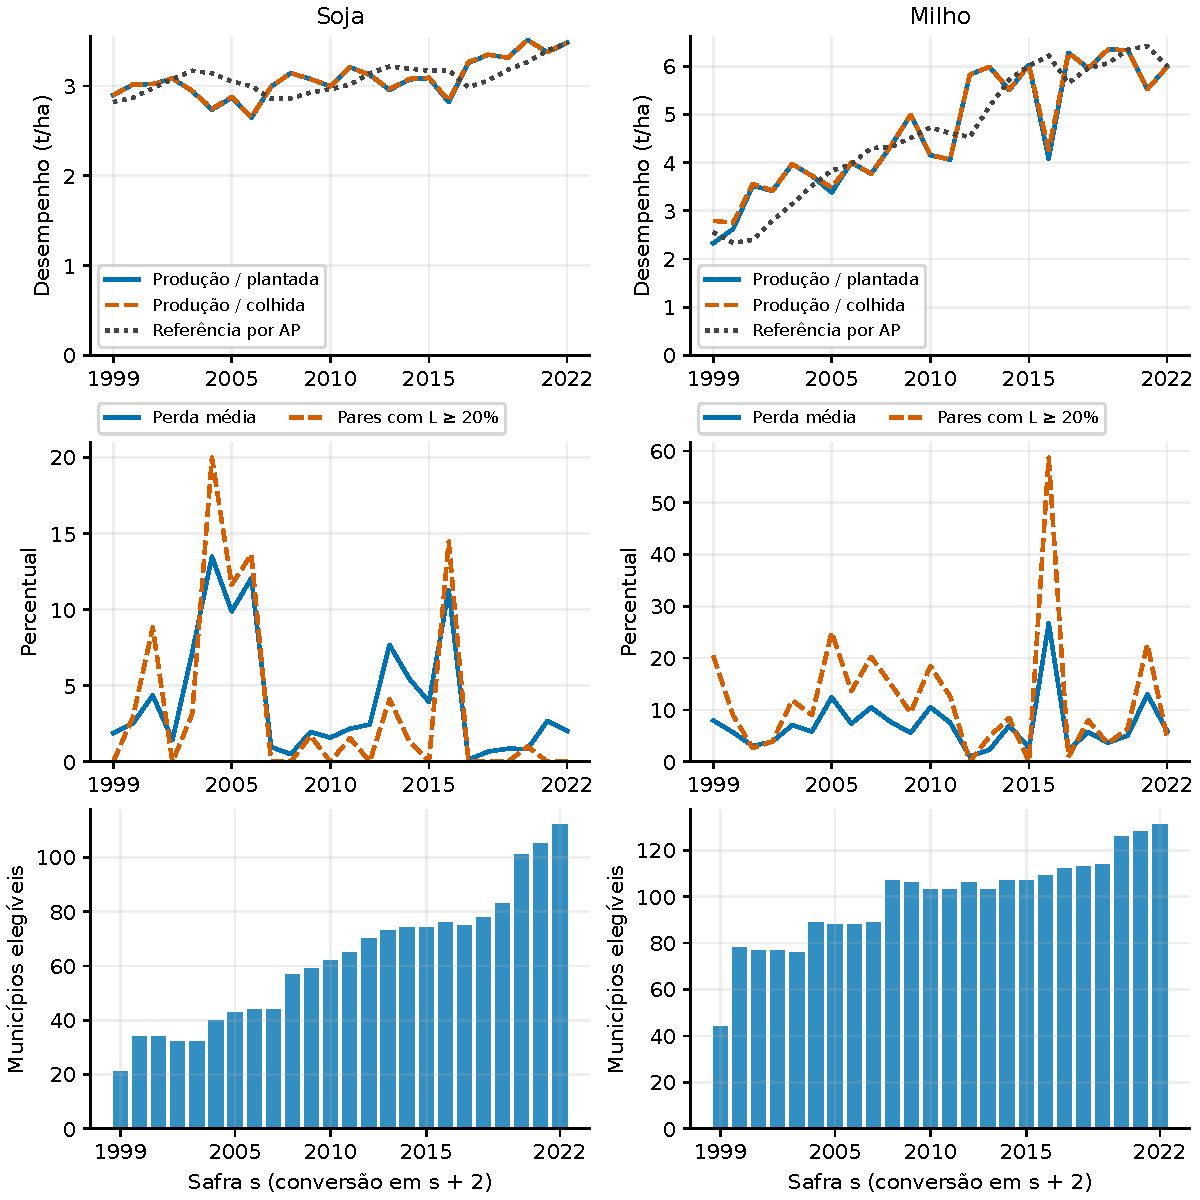
\includegraphics[width=\textwidth]{assets/fig10_perdas_desempenho_etapa5.pdf}
\caption{Desempenho agrícola, perdas anteriores e cobertura das amostras}
\label{fig:h1b-perdas}
\begin{minipage}{\textwidth}\footnotesize\centering
Fonte: elaboração própria com IBGE/PAM e MapBiomas 10.1.
\end{minipage}
\end{figure}
\FloatBarrier

Em 2016, por exemplo, a amostra de milho apresentou 4,08 t/ha plantado e 4,26 t/ha colhido, diante de referência ponderada de 6,22 t/ha. A perda municipal média foi 26,7\%, e 58,7\% dos 109 municípios elegíveis registraram déficit de pelo menos 20\%. A comparação reúne menor desempenho nas áreas colhidas e não colheita de parte da área plantada, sem identificar a causa. A cobertura muda entre safras; suas médias não descrevem a evolução do risco em um grupo fixo. Essa condição é relevante tanto para interpretar as trajetórias quanto para definir as observações que podem entrar em H1b.

Na Tabela~\ref{tab:h1b-composicao}, cada célula apresenta média e mediana, com igual peso aos pares município--ano. A coluna observada reúne os 2.772 pares de conversão; soja e milho são subconjuntos sobrepostos com perda anterior válida. As taxas usam o estoque nativo inicial, e os potenciais fixos reaparecem em cada ano observado. A conversão agrícola média é menor nos subconjuntos elegíveis, sobretudo no milho. A tabela antecipa, assim, que incluir perdas modifica também a composição da amostra. A chuva caracteriza outra condição variável no tempo: sua anomalia anual, em milímetros, compara a precipitação com a média municipal de 1981--2000, utilizando CHIRPS. Ela não corresponde diretamente ao clima da safra anterior.

\begin{table}[htbp]
\centering\small\captionstyle{\centering}\normalcaption
\caption{Composição da amostra observada e das amostras com perdas anteriores}\label{tab:h1b-composicao}
\begin{tabular}{lrrr}
\hline
Indicador & Observada & Soja & Milho \\
\hline
Pares município--ano & 2.772 & 1.488 & 2.381 \\
Municípios & 137 & 115 & 137 \\
Conversão agrícola (\%) & 0,112 (0,014) & 0,106 (0,029) & 0,085 (0,013) \\
Conversão para pastagem (\%) & 1,192 (0,799) & 0,943 (0,701) & 1,142 (0,765) \\
Potencial da soja (kg MS/ha) & 2.942 (2.837) & 2.981 (2.950) & 2.965 (2.916) \\
Potencial do milho (kg MS/ha) & 3.245 (3.135) & 3.177 (3.066) & 3.269 (3.144) \\
Anomalia de chuva em t (mm) & -31,4 (-36,4) & -33,3 (-43,7) & -33,3 (-41,2) \\
\hline
\end{tabular}
\par\smallskip\begin{minipage}{\textwidth}\footnotesize\centering
Fonte: elaboração própria com MapBiomas, IBGE/PAM, GAEZ v4 e CHIRPS.
\end{minipage}
\end{table}

\FloatBarrier

Os dados de produção, comércio e autuações complementam essa contextualização no Texto~\ref{S-text:s2}. Não são usados como substitutos da conversão ou da exposição institucional. Exportações por domicílio fiscal não localizam a área produtora; contagens administrativas dependem de cobertura, detecção e classificação das infrações. Ao preservar essas distinções, a descrição fornece uma base para a análise das associações, sem atribuir aos agregados decisões individuais que não foram observadas.

\section{Estratégia empírica}
\label{sec:estrategia}

\subsection{Conversão, perdas e ordenação temporal}

A variável dependente é a taxa anual de conversão bruta da vegetação nativa para agricultura. Para o município $i$ e o ano $t$, divide-se a área dessa transição pelo estoque nativo em $t-1$, multiplicando-se por cem. A unidade é ponto percentual (p.p.) do estoque inicial. A mesma construção define o desfecho complementar de pastagem. Ao observar diretamente as transições, a medida evita que regeneração em outras parcelas compense a abertura do ano, como ocorreria numa diferença líquida entre estoques. O destino registrado é o uso imediatamente posterior à vegetação; a classificação não informa a cultura plantada, a legalidade da abertura ou os agentes que a realizaram.

A quebra é construída separadamente para cada cultura $c$, comparando o desempenho realizado com uma referência histórica municipal. Utiliza-se $r^c_{is}=Q^c_{is}/AP^c_{is}$, em que $Q$ é a produção e $AP$, a área plantada na safra anual $s$. Quando as áreas são positivas, essa razão pode ser escrita como rendimento por hectare colhido multiplicado pela proporção colhida da área plantada. Essa decomposição dá sentido à escolha: um município pode apresentar perda mesmo que o rendimento das parcelas que chegaram à colheita se mantenha. A medida também pode variar com manejo, composição de áreas ou erro de declaração, de modo que seu déficit não equivale automaticamente a dano climático.

A referência $\widehat r^c_{is}$ resulta de uma tendência linear estimada com os dez anos anteriores a $s$, exigindo pelo menos sete observações válidas e previsão positiva. A tendência admite evolução gradual do desempenho, ao passo que a janela móvel limita a influência de um passado produtivo distante. Nenhuma observação futura participa da previsão. Descontinuidades territoriais identificadas reiniciam o histórico, evitando que a mudança da unidade seja interpretada como perda. A intensidade é definida por:
\begin{equation}
L^c_{is}=\max\left\{0,\,1-\frac{r^c_{is}}{\widehat r^c_{is}}\right\}.
\label{eq:perda}
\end{equation}
Assim, $L=0,20$ indica desempenho 20\% abaixo da referência local, e realizações acima dela recebem zero na especificação principal. Ausência de cultivo e informação insuficiente permanecem sem perda calculada. Uma versão binária identifica déficits de pelo menos 20\%; alternativas de janela, referência e limiar examinam a sensibilidade a essas escolhas no Texto~\ref{S-text:s4}. A referência é uma estimativa, e não uma produtividade que teria sido observada com certeza na ausência de choque.

O alinhamento principal associa a transição dos mapas entre $t-1$ e $t$ à perda da safra $t-2$ e ao preço médio de $t-1$. Para a conversão de 2001, por exemplo, utiliza-se a perda de 1999, cuja referência pode mobilizar 1989--1998, e o preço de 2000. Para 2024, utilizam-se perda de 2022 e preço de 2023. A separação reduz a sobreposição entre o desempenho medido e a abertura que se pretende descrever, mas os dados anuais não permitem ordenar todas as decisões dentro de cada ano. A PAM agrega as safras de milho, e os mapas não datam cada supressão. A alternativa com perda em $t-1$ é, por isso, uma verificação distinta, sujeita a maior sobreposição temporal.

Define-se $p^c_{t-1}$ como o logaritmo do preço real, centrado na média dos 24 valores anuais usados no painel. A capacidade $Z^c_i$ é padronizada pela média e pelo desvio-padrão dos 141 municípios, conservados em todas as amostras. Essa padronização permite comparar coeficientes sem que a unidade de capacidade mude quando municípios são excluídos. Uma variação de 10\% no preço corresponde a $\ln(1,10)$ na escala logarítmica. O modelo em nível do logaritmo relaciona o patamar real do incentivo à conversão; a variação anual e a razão entre preços respondem a perguntas diferentes e entram apenas como alternativas identificadas separadamente.

\subsection{Contrastes de capacidade e perdas}

O núcleo procura distinguir duas formas de heterogeneidade. A primeira compara a associação com preços entre municípios de diferentes capacidades potenciais; a segunda compara essa associação diante de diferentes perdas anteriores. Para cada cultura, estima-se:
\begin{equation}
\begin{split}
y^{ag}_{it}={}&\alpha_i+\lambda_{b(i),t}
 +\beta_c p^c_{t-1}Z^c_i
 +\theta_c L^c_{i,t-2}
 +\delta_c p^c_{t-1}L^c_{i,t-2}\\
 &+\gamma_c Z^c_i\tau_t+\rho_c R_{it}+\varepsilon^c_{it},
\end{split}
\label{eq:nucleo}
\end{equation}
em que $\alpha_i$ são efeitos municipais, $\lambda_{b(i),t}$ são efeitos do bioma predominante por ano, $\tau_t=(t-2001)/10$ e $R_{it}$ é a anomalia anual de precipitação, em centenas de milímetros. Os efeitos municipais absorvem características locais constantes; os de bioma por ano absorvem choques comuns aos municípios de cada grupo no mesmo ano. A tendência diferenciada por capacidade permite que municípios de maior potencial sigam trajetória gradual distinta, além da associação com o preço. A chuva representa uma condição contemporânea que pode afetar diretamente vegetação e conversão, sem ser utilizada como instrumento para a perda.

Os níveis isolados de preço e capacidade não aparecem porque são absorvidos pelos efeitos fixos. Sua interação continua identificável se houver variação suficiente de capacidade entre municípios e de preços ao longo do tempo, após os demais termos. A perda varia nas duas dimensões e permanece na equação junto com preço×perda. O parâmetro $\theta_c$ descreve sua associação no preço centrado igual a zero; H1b se refere a $\delta_c$, que altera a inclinação em relação ao preço. A presença de uma associação entre perda e conversão, sem essa interação, não seria um teste da sub-hipótese.

Para H1a, o contraste entre municípios separados por um desvio-padrão de capacidade, diante de uma alta de 10\% no preço, é $\beta_c\ln(1,10)$ p.p. A hipótese prevê $\beta_c>0$. Para H1b, a diferença associada a dez pontos percentuais adicionais de perda é $\delta_c\ln(1,10)\times0,10$ p.p.; seu sinal é uma questão empírica. Esses contrastes não recuperam o efeito médio de uma alta de preços em Mato Grosso, absorvido pelos efeitos temporais. Eles descrevem diferenças condicionais de associação, com as demais variáveis da equação mantidas constantes.

A especificação B corresponde à Equação~\ref{eq:nucleo}. A especificação A exclui os dois termos de perda e é estimada tanto na amostra disponível originalmente quanto nas mesmas chaves de B. A comparação entre A original e A comum identifica a alteração associada ao recorte, enquanto A comum e B mostram a alteração decorrente da inclusão dos termos, conservando as observações. A amostra elegível pela perda contém 1.488 pares na soja e 2.381 no milho. A remoção de grupos unitários sem contribuição à estimação com esses efeitos fixos deixa, respectivamente, 1.459 pares em 106 municípios e 2.376 em 134. A original reúne 2.767 pares em 134 municípios. A versão com limiar de 20\% utiliza as mesmas chaves de B.

Essa distinção é relevante para o alcance territorial. No Pantanal, B dispõe de oito pares em dois municípios para soja e cinquenta em três para milho. O painel não fornece base comparável à dos demais biomas para interpretar uma resposta própria dessa região. O histórico também seleciona localidades com cultivo e registro suficientemente contínuos. A análise das perdas diz respeito a esse conjunto, sem representar integralmente municípios de entrada recente na agricultura ou unidades sem informação válida. As tabelas de composição e suporte do suplemento permitem acompanhar essa seleção antes de atribuir diferenças à resposta econômica.

\subsection{Inferência e verificações de estabilidade}

A multiplicação dos preços anuais por características municipais amplia a variação das interações, mas não cria novos choques independentes de preço. Apresentam-se três procedimentos de inferência: agrupamento por município, agrupamento simultâneo por município e ano e HAC com banda dois sobre os escores anuais da regressão completa residualizada. Neste último, a aplicação de Frisch--Waugh--Lovell preserva os coeficientes de B; utilizam-se pesos de Bartlett, sem pré-branqueamento ou ajuste adicional de pequena amostra. Os graus de liberdade são, respectivamente, $G-1$, $\min(G,T)-1$ e $T-1$, em que $G$ é o número de municípios e $T$, o de anos. Com 24 anos, as duas últimas referências utilizam 23 graus de liberdade.

O agrupamento municipal admite dependência serial dentro da unidade; o agrupamento duplo acrescenta dependência entre municípios no mesmo ano. O HAC dos escores anuais examina a persistência temporal da contribuição agregada à estimação. Nenhum procedimento garante acomodar toda forma de dependência espacial e temporal, especialmente com poucos anos e interações concentradas. Por isso, a apresentação conserva a divergência entre as inferências. Intervalos são de 95\%, e ajustes de Holm são aplicados a famílias explicitadas: os dois gradientes H1a de B, separadamente dos dois modificadores H1b. Nas extensões, as famílias acompanham o conjunto de contrastes efetivamente examinado; os intervalos apresentados continuam individuais.

As verificações incluem dezesseis definições por cultura, com variações da referência produtiva, intensidade ou ocorrência da perda, calendário, clima, efeitos temporais, tendência por capacidade, janela e preço. Comparações intermediárias nas mesmas chaves separam, quando necessário, modificação da fórmula de alteração de amostra. Também se examinam exclusões locais e anuais, reamostragem restrita por ano e perturbações da referência histórica. Essas últimas verificam a sensibilidade ao indicador gerado, sem converter sua distribuição em intervalo que incorpore toda a incerteza do desenho. Os procedimentos completos e seus resultados encontram-se nos Textos~\ref{S-text:s4} e~\ref{S-text:s5}.

Três períodos --- 2001--2005, 2006--2011 e 2012--2024 --- permitem verificar se uma associação agregada esconde trajetórias distintas. Interagem-se os termos de interesse com os períodos, preservando os constitutivos e os ajustes de tendência previstos na especificação. Os testes conjuntos examinam tanto a nulidade dos modificadores quanto sua igualdade entre períodos. São comparações exploratórias: os períodos iniciais contêm poucos preços e poucas perdas intensas, sobretudo na soja. Seu uso não transforma as datas em mudanças exógenas ou em avaliação de políticas.

\subsection{Destinos, incentivos conjuntos e instituições}

A extensão para pastagem conserva fórmula e observações de B. A diferença agricultura menos pastagem é estimada diretamente, de modo que sua variância incorpora a covariância entre os destinos. Outra extensão acrescenta a interação entre capacidade e perda e a interação tripla entre preço, capacidade e perda, permitindo que a modificação de H1b também varie com o potencial. Os dois termos entram juntos para respeitar a hierarquia da interação. Os contrastes condicionais são avaliados na distribuição observada; percentis marginais não asseguram observações em todas as combinações de capacidade e perda.

O preço relativo é $\ln[P^c/(1000P^{carne})]$, com o fator mil compatibilizando cotações por tonelada e por quilograma. Essa medida compara incentivos brutos entre produtos, sem descontar custos. Testa-se a restrição de coeficientes opostos que ela impõe a uma versão com preços separados. Estima-se ainda uma versão conjunta de soja e milho na interseção de 1.450 pares em 105 municípios, mantendo referências individuais nessas mesmas chaves. A correlação de 0,948 entre as séries de preços justifica cautela ao separar sua contribuição, mesmo quando a matriz de interações mantém posto completo.

A exposição territorial à Moratória utiliza a fração municipal no bioma Amazônia interagida com o período desde 2007, com alternativa desde 2006. O pacto foi anunciado em julho de 2006; a alteração do marco de desmatamento para julho de 2008 ocorreu em dezembro de 2014. Nenhuma dessas datas equivale a um início uniforme de cumprimento municipal. A medida representa alcance potencial do compromisso sobre a soja, sem observar fornecedores e transações; para milho, caracteriza heterogeneidade no território alcançado pelo pacto de outra cultura.

Para a reforma do Código Florestal, utiliza-se a fração de formações florestais de 2000 na área municipal total, inclusive municípios com valor zero, combinada ao período desde 2013 e, alternativamente, desde 2012. A medida reúne classes 3 e 6 do MapBiomas e não corresponde a percentual jurídico de Reserva Legal, passivo ou situação cadastral. As extensões institucionais acrescentam, separadamente, preço×capacidade×exposição×pós e preço×perda×exposição×pós, com todos os termos de ordem inferior que não são absorvidos e tendência pela exposição. As equações completas estão no Texto~\ref{S-text:s5}. Sua interpretação depende da variação residual disponível e da possibilidade de outras mudanças acompanharem a exposição e a data.

O desenho permanece associativo. Preços internacionais não medem o retorno líquido recebido localmente; clima, infraestrutura, tecnologia e composição produtiva podem variar junto com as interações. A defasagem da perda ordena medidas, mas não elimina choques persistentes ou decisões anteriores que afetem simultaneamente desempenho e conversão. Controles como crédito, renda e produção posteriores à quebra poderiam representar consequências do próprio evento, alterando o contraste. Fiscalização observada também pode responder à pressão de abertura. Esses limites orientam a escolha do núcleo parcimonioso e a interpretação das extensões, sem supor que acrescentar controles produza automaticamente identificação causal.

\section{Resultados}
\label{sec:resultados}

\subsection{Composição da amostra e contrastes principais}

A Tabela~\ref{tab:h1-principais} mostra que parte relevante da mudança de H1a antecede a inclusão das perdas. Na soja, o gradiente preço×capacidade passa de 0,08484 em A original a 0,04645 em A comum; no milho, de 0,05188 a 0,03090. Ao acrescentar intensidade e interação, B apresenta valores próximos aos da referência comum. A redução, portanto, não pode ser atribuída integralmente a um ajuste por quebra de safra. Ela acompanha a seleção de municípios e anos com histórico produtivo suficiente, cuja diferença de conversão média já aparecia na análise descritiva.

% Gerado por etapa9/publicar_tabelas.py; fontes e células registradas na auditoria.
\begin{table}[htbp]
\centering
\small
\setlength{\tabcolsep}{3pt}
\renewcommand{\arraystretch}{1.1}
\normalcaption\captionstyle{\centering}
\caption{Conversão para agricultura: capacidade e perdas anteriores}
\label{tab:h1-principais}
\begin{tabular}{lccc}
\hline
Variável & A original & A comum & B: intensidade \\
\hline\multicolumn{4}{l}{\textbf{Soja}} \\
$pZ$ & 0,08484 & 0,04645 & 0,04043 \\
 & (0,03578) & (0,05183) & (0,05307) \\
$L$ & -- & -- & -0,13128 \\
 &  &  & (0,06165) \\
$pL$ & -- & -- & 0,42338 \\
 &  &  & (0,29654) \\
$Z\tau$ & 0,04050 & 0,03728 & 0,03610 \\
 & (0,01444) & (0,02365) & (0,02380) \\
$R$ & -0,01348 & -0,00643 & -0,00650 \\
 & (0,00626) & (0,00437) & (0,00437) \\
Pares município--ano & 2.767 & 1.459 & 1.459 \\
Municípios & 134 & 106 & 106 \\
$R^2$ total & 0,3828 & 0,5109 & 0,5119 \\
$R^2$ \textit{within} & 0,0198 & 0,0159 & 0,0180 \\
\hline\multicolumn{4}{l}{\textbf{Milho}} \\
$pZ$ & 0,05188 & 0,03090 & 0,03218 \\
 & (0,01787) & (0,01823) & (0,01820) \\
$L$ & -- & -- & 0,04491 \\
 &  &  & (0,03955) \\
$pL$ & -- & -- & -0,01315 \\
 &  &  & (0,11571) \\
$Z\tau$ & 0,05382 & 0,05062 & 0,05080 \\
 & (0,01517) & (0,01791) & (0,01781) \\
$R$ & -0,01516 & -0,00322 & -0,00310 \\
 & (0,00671) & (0,00342) & (0,00344) \\
Pares município--ano & 2.767 & 2.376 & 2.376 \\
Municípios & 134 & 134 & 134 \\
$R^2$ total & 0,3807 & 0,4213 & 0,4217 \\
$R^2$ \textit{within} & 0,0165 & 0,0184 & 0,0190 \\
\hline\end{tabular}
\par\smallskip
\begin{minipage}{\textwidth}\footnotesize\centering
Fonte: elaboração própria com MapBiomas 10.1, IBGE/PAM, GAEZ v4, Banco Mundial, CPI-U e CHIRPS.
\end{minipage}
\end{table}


Os coeficientes estão na escala da equação, e os valores entre parênteses são erros-padrão com agrupamento municipal. Todas as colunas incluem os efeitos municipais e de bioma por ano, a tendência por capacidade e a anomalia de chuva. O $R^2$ total incorpora a contribuição dos efeitos fixos, enquanto o indicador \textit{within} se refere à variação após sua absorção. A comparação desses ajustes entre amostras diferentes não constitui medida de superioridade da explicação econômica. A leitura substantiva se concentra nos contrastes e em sua precisão sob as três inferências.

Em B, os gradientes de H1a continuam positivos nas duas culturas, mas os intervalos de 95\% abrangem zero. O modificador de H1b é positivo na soja e próximo de zero, com sinal negativo, no milho; seus intervalos também abrangem zero nos três procedimentos. A versão binária com limiar de 20\% não produz contraste preciso. A Tabela~\ref{tab:h1-magnitudes} apresenta os intervalos dos contrastes principais, e a Tabela~\ref{S-tab:h1-ocorrencia-etapa9}, a alternativa binária. Esses resultados preservam a direção prevista para a capacidade no núcleo, sem confirmar sua positividade de forma geral; para as perdas, não permitem estabelecer uma modificação estável nem concluir que ela inexista.

\FloatBarrier
A associação isolada da perda ajuda a esclarecer a diferença entre nível e interação. Na soja, seu coeficiente é negativo e rejeita zero com agrupamento municipal, mas não com agrupamento duplo ou HAC. Como o preço foi centrado, esse coeficiente se refere à associação da perda no patamar médio do logaritmo do preço. Mesmo que fosse preciso nos três casos, ele não demonstraria restrição financeira nem substituiria o contraste preço×perda. A mudança de precisão reforça a necessidade de distinguir o parâmetro examinado da narrativa que poderia explicá-lo.

% Gerado por etapa9/publicar_tabelas.py; fontes e células registradas na auditoria.
\begin{table}[htbp]
\centering
\footnotesize
\setlength{\tabcolsep}{3pt}
\renewcommand{\arraystretch}{1.1}
\normalcaption\captionstyle{\centering}
\caption{Contrastes de capacidade e perda para aumento de 10\% no preço (p.p.)}
\label{tab:h1-magnitudes}
\begin{tabular}{lcccc}
\hline
Cultura / hipótese & Estimativa & IC95 mun. & IC95 mun.+ano & IC95 HAC(2) \\
Soja / H1a & 0,00385 & [-0,00618; 0,01388] & [-0,00666; 0,01437] & [-0,00273; 0,01044] \\
Soja / H1b & 0,00404 & [-0,00157; 0,00964] & [-0,00452; 0,01259] & [-0,00517; 0,01324] \\
Milho / H1a & 0,00307 & [-0,00036; 0,00650] & [-0,00139; 0,00752] & [-0,00075; 0,00688] \\
Milho / H1b & -0,00013 & [-0,00231; 0,00206] & [-0,00211; 0,00186] & [-0,00110; 0,00085] \\
\hline\end{tabular}
\par\smallskip
\begin{minipage}{\textwidth}\footnotesize\centering
Fonte: elaboração própria com MapBiomas 10.1, IBGE/PAM, GAEZ v4, Banco Mundial, CPI-U e CHIRPS.
\end{minipage}
\end{table}

\FloatBarrier

A Tabela~\ref{tab:h1-magnitudes} traduz os coeficientes para uma alta de 10\% no preço, combinada a um desvio-padrão adicional de capacidade ou a dez pontos percentuais adicionais de perda. Para H1b, os contrastes são 0,00404 p.p. na soja e $-0,00013$ p.p. no milho. Com agrupamento duplo, os intervalos são $[-0,00452;\,0,01259]$ e $[-0,00211;\,0,00186]$ p.p. A unidade refere-se ao estoque nativo inicial, e não à variação percentual da área agrícola. As taxas médias de conversão nas amostras de B são 0,10810 e 0,08506 p.p.; elas contextualizam a escala, mas a divisão de um contraste por essas médias não o transforma em efeito causal proporcional.

\subsection{Estabilidade temporal e informação disponível}

As alternativas não revelam uma definição de perda que sustente H1b uniformemente. Nenhum dos dezesseis modificadores por cultura rejeita zero após o ajuste de Holm, em qualquer das três inferências. Há resultados pontualmente mais precisos: na soja, a janela desde 2006 produz modificador negativo e rejeição bruta no agrupamento duplo e no HAC. Após o ajuste na família, os p-valores passam a 0,5557 e 0,4161. O sinal oposto ao núcleo é preservado nas Tabelas~\ref{S-tab:h1-sens-soja} e~\ref{S-tab:h1-sens-milho}; não é descartado como anomalia nem escolhido como resultado principal.

A decomposição por períodos explicita essa instabilidade. Na soja, preço×perda é positivo em 2001--2005 e negativo nos dois períodos seguintes; no milho, é negativo no primeiro e pequeno nos demais. Os testes de nulidade conjunta e igualdade dos modificadores rejeitam com HAC após Holm nas duas culturas, sem uniformidade entre os procedimentos. Para H1a, o gradiente da soja em 2012--2024 é negativo, com intervalo de agrupamento duplo inteiramente abaixo de zero. Esse resultado contraria a direção da sub-hipótese naquele recorte e deve acompanhar a interpretação dos sinais positivos do núcleo. A Tabela~\ref{S-tab:h1-regimes-etapa9} apresenta os coeficientes e o suporte correspondente.

A informação desses contrastes está distribuída de forma desigual. Os períodos iniciais contêm cinco e seis preços anuais, e a soja reúne apenas cinco ocorrências de perda de pelo menos 20\% no primeiro. Na inferência HAC, mudar a banda entre zero e quatro mantém as rejeições brutas dos testes da soja; no milho, elas dependem da banda. Em B, Jangada em 2013, associada à safra de 2011, concentra 29,85\% da soma de quadrados residualizada de preço×perda da soja. Excluir esse par eleva o modificador, ainda impreciso; retirar 2003 muda seu sinal. A influência é documentada sem eliminar observações para obter uma direção desejada.

As verificações adicionais mantêm a incerteza. A reamostragem restrita por ano, com 999 replicações, produz p-valores de 0,603 e 0,877 para os modificadores de soja e milho. Nas 499 perturbações da referência histórica por cultura, os quantis de 2,5\% e 97,5\% também atravessam zero. São sensibilidades condicionais à construção do indicador, não intervalos que resolvem toda a incerteza. Na alternativa que substitui o preço defasado pelo futuro, o gradiente preço×capacidade do milho é positivo nas três inferências. Esse comportamento, limitado ao período com preço futuro disponível, recomenda cautela diante de tendências persistentes; não demonstra antecipação ou expectativa dos produtores.

\subsection{Destinos e extensões do contraste}

A Tabela~\ref{tab:h1-destinos-robustez} compara agricultura e pastagem nas mesmas observações de cada cultura. Os gradientes preço×capacidade são maiores para pastagem. A diferença entre destinos é imprecisa na soja e rejeita zero nos p-valores brutos das três inferências no milho. Neste último caso, +10\% no preço e um desvio-padrão adicional de capacidade correspondem a uma diferença de $-0,04315$ p.p. entre os gradientes de agricultura e pastagem. Na família de quatro contrastes, contudo, o p-valor ajustado permanece abaixo de 5\% apenas com agrupamento municipal. As diferenças de preço×perda são imprecisas mesmo antes do ajuste.

% Gerado por etapa9/publicar_tabelas.py; fontes e células registradas na auditoria.
\begin{table}[htbp]
\centering
\footnotesize
\setlength{\tabcolsep}{3pt}
\renewcommand{\arraystretch}{1.1}
\normalcaption\captionstyle{\centering}
\caption{Gradientes por destino da conversão e diferença entre destinos}
\label{tab:h1-destinos-robustez}
\begin{tabular}{lcccc}
\hline
Destino & $\beta$ & IC95 de $\beta$ & $\delta$ & IC95 de $\delta$ \\
\hline\multicolumn{5}{l}{\textbf{Soja}} \\
Agricultura & 0,04043 & [-0,0699; 0,1508] & 0,42338 & [-0,4743; 1,3211] \\
Pastagem & 0,21472 & [-0,0065; 0,4360] & 0,28650 & [-3,2205; 3,7935] \\
Agricultura--pastagem & -0,17429 & [-0,4297; 0,0811] & 0,13688 & [-4,0375; 4,3112] \\
\hline\multicolumn{5}{l}{\textbf{Milho}} \\
Agricultura & 0,03218 & [-0,0145; 0,0789] & -0,01315 & [-0,2218; 0,1955] \\
Pastagem & 0,48490 & [0,0647; 0,9051] & -1,18909 & [-3,6083; 1,2302] \\
Agricultura--pastagem & -0,45272 & [-0,8824; -0,0231] & 1,17594 & [-1,2361; 3,5879] \\
\hline\end{tabular}
\par\smallskip
\begin{minipage}{\textwidth}\footnotesize\centering
Fonte: elaboração própria com MapBiomas 10.1, IBGE/PAM, GAEZ v4, Banco Mundial, CPI-U e CHIRPS.
\end{minipage}
\end{table}

\FloatBarrier

Os intervalos dessa tabela utilizam agrupamento por município e ano. O potencial permanece o da cultura, inclusive na equação de pastagem. A comparação permite reconhecer que os dois destinos apresentam associações diferentes em algumas especificações, sem converter capacidade agrícola em capacidade pecuária. Também não acompanha o deslocamento de atividades entre parcelas ou municípios. Os testes completos, incluindo a diferença estimada diretamente, constam da Tabela~\ref{S-tab:h1-inferencia-extra}.

A interação tripla com capacidade não torna H1b mais conclusiva. Seus coeficientes são positivos na soja e negativos no milho, mas nenhum dos seis testes da família rejeita após Holm nas três inferências. Os contrastes condicionais nos percentis de capacidade têm intervalos de agrupamento duplo que abrangem zero. Os intervalos dos gradientes com preço relativo à carne também abrangem zero. As restrições de coeficientes opostos não são rejeitadas, o que não estabelece equivalência entre medidas. Na amostra compartilhada pelas culturas, a inclusão conjunta não produz rejeição dos testes conjuntos de H1a ou H1b. As Tabelas~\ref{S-tab:h1-extensoes-etapa9}, \ref{S-tab:h1-cenarios-tripla} e~\ref{S-tab:h1-conjunto-etapa9} conservam essas comparações.

\subsection{Heterogeneidade em torno dos marcos institucionais}

Nas datas principais, nenhum dos oito contrastes institucionais rejeita após Holm com agrupamento municipal ou duplo. No HAC, a interação de preço, perda, fração amazônica e período desde 2007 para o milho é negativa e mantém rejeição ajustada, assim como a alternativa desde 2006. Para +10\% no preço, +0,10 na perda e +0,10 na fração amazônica, o primeiro contraste equivale a $-0,00891$ p.p. na diferença pós--pré. A rejeição restrita ao HAC é apresentada como parte da evidência, sem ser tomada como concordância entre procedimentos. As dezesseis versões estão nas Tabelas~\ref{S-tab:h1-instituicoes-principal} e~\ref{S-tab:h1-instituicoes-alternativa}.

A variação que sustenta esse contraste é estreita. Depois dos demais termos, permanece apenas 0,453\% da soma de quadrados da interação do milho após os efeitos fixos; um município concentra 19,0\% da variação parcial, e 2005, 41,9\%. As dezesseis matrizes institucionais de agrupamento duplo e a do modelo conjunto exigiram correção de autovalores negativos. O procedimento conserva os coeficientes e viabiliza os intervalos, mas não amplia a informação disponível. Na comparação pela cobertura florestal inicial em torno de 2012, o contraste H1a da soja é negativo, com rejeições brutas que não persistem após Holm. As demais estimativas e a mudança de resultados entre datas estão preservadas no suplemento.

\section{Discussão e implicações para a gestão ambiental}
\label{sec:discussao}
\label{discussao-margens}

\subsection{Incentivos econômicos e possibilidades de expansão}

O primeiro resultado substantivo diz respeito ao alcance da associação estimada. A exigência de histórico produtivo reduz os gradientes preço×capacidade antes da introdução das perdas. Isso aproxima a leitura econométrica da descrição das amostras: localidades com informação suficientemente longa não constituem uma reprodução proporcional de todo o território observado. Como entrada no cultivo, continuidade de produção e disponibilidade de registros participam da seleção, a estimativa com perdas não pode ser lida como atualização neutra da mesma população. A contribuição da comparação entre A original, A comum e B está em tornar visível essa diferença, que poderia ser confundida com evidência de um mecanismo econômico.

A direção positiva dos gradientes de capacidade em B é compatível com a ideia de que uma valorização da cultura aumenta mais a receita potencial por hectare em locais produtivamente favorecidos. A imprecisão, entretanto, impede estabelecer essa relação de forma geral no recorte com histórico. A comparação com \citeonline{BermanEtAl2023} deve considerar que seu desenho, território e suporte de variação diferem dos utilizados aqui. Acrescentar perdas a um painel municipal não constitui, por si só, demonstração de um mecanismo ausente naquele estudo. O avanço específico está na distinção entre capacidade potencial, desempenho anterior e destino da conversão, acompanhada da verificação de quanto o resultado depende da composição e da inferência.

Essa distinção também limita a interpretação tecnológica. O potencial sob alto insumo e sequeiro representa uma possibilidade padronizada; não informa o insumo utilizado nas parcelas convertidas. Nos modelos antecedentes preservados na Tabela~\ref{S-tab:h1-margens-tecnologia}, a associação positiva do cenário de alto insumo não se reproduz sob baixo insumo e se torna negativa com o índice de adequação. A ocupação agrícola anterior apresenta relação distinta do potencial. Esses resultados qualificam a leitura de H1a, em consonância com a heterogeneidade das respostas à intensificação discutida por \citeonline{Spera2017}. Como não incluem o contraste com perdas, permanecem antecedentes de H1a e não evidência de H1b.

A comparação entre destinos ajuda a compreender por que produção e conversão não caminham necessariamente juntas. A substituição de pastagens por lavouras pode ampliar a produção sem abertura imediata de vegetação, enquanto novas pastagens podem surgir em outras áreas. \citeonline{MacedoEtAl2012} documentaram a importância de terras previamente abertas para a expansão da soja na porção florestal de Mato Grosso; \citeonline{Braganca2018} mostrou que preços relativos podem se associar a reorganização de usos sob condições particulares. O maior gradiente da pastagem em parte das estimativas é compatível com a relevância de examinar esses destinos em conjunto, mas não identifica a sequência de realocação descrita por tais mecanismos. As interdependências discutidas por \citeonline{SimoesEtAl2020} e \citeonline{JungEtAl2022} exigem informações que ultrapassam o destino municipal imediato.

Para a gestão ambiental, a implicação é acompanhar o caminho da expansão, além do volume produzido. O crescimento da safra pode resultar de rendimento, frequência de cultivo, substituição de uso ou incorporação de novas áreas; cada margem envolve pressões distintas. Uma leitura apoiada apenas em produção ou área agrícola líquida pode reunir processos opostos. Os dados de transição bruta oferecem uma medida mais próxima da abertura observada, mas ainda precisam ser relacionados às parcelas, à sequência de usos e às regras aplicáveis para sustentar decisões operacionais. O artigo não estima um limiar de preço para acionar fiscalização nem classifica municípios por risco previsto.

\subsection{Perdas anteriores e mecanismos ainda em aberto}

A formulação sem sinal prévio de H1b encontra respaldo na diversidade de respostas possíveis, e não na equivalência de todas as explicações. Uma quebra pode reduzir recursos próprios, alterar acesso ao crédito e adiar investimento; também pode ser seguida de expansão se houver condições para financiar a atividade ou reorganizar a produção. O painel não observa essas decisões nem identifica qual restrição foi determinante. Por isso, o sinal positivo da interação na soja não prova recuperação de renda por abertura, assim como o sinal negativo em recortes posteriores não demonstra falta de liquidez. Essas interpretações permanecem hipóteses sobre processos que poderiam produzir as associações.

A literatura oferece evidências para componentes dessa discussão. \citeonline{AssuncaoEtAl2020Credito} identificaram consequências do condicionamento do crédito para o desmatamento, com heterogeneidade entre atividades; \citeonline{KarlanEtAl2014} distinguiram a importância de seguro e capital para investimento em outro contexto agrícola. Tais resultados justificam considerar finanças e risco, mas não autorizam atribuir a cada déficit municipal uma restrição financeira. A intensidade da perda física tampouco mede perda de receita: preços locais, custos, estoques, contratos e proteção financeira podem alterar sua transmissão. O indicador $Q/AP$ é adequado para descrever desempenho por área comprometida com o cultivo, preservando essa separação em relação ao resultado econômico.

Os estudos mais próximos de perdas e mudança de uso também recomendam especificar a margem observada. Em \citeonline{OrdonezEtAl2025}, a precisão da expansão de lavouras diferiu entre o painel de famílias e a análise espacial; a produção de carvão constituiu outra resposta. Em \citeonline{HsiaoEtAl2026}, o aumento de preços locais no Brasil acompanhou a redução da produtividade física sob calor extremo. Esses resultados mostram que a ligação entre choque produtivo e pressão sobre a vegetação depende do mercado e da unidade de observação. Aqui, preços internacionais comuns, perda histórica municipal e conversão posterior compõem um contraste diferente, cuja imprecisão não refuta aqueles mecanismos em seus contextos originais.

A heterogeneidade temporal merece ser mantida nesse diálogo. O modificador da soja muda de sinal após o primeiro período, e seu gradiente de capacidade torna-se negativo no período final. Esses resultados dificultam uma interpretação de resposta única ao longo de duas décadas. Ao mesmo tempo, poucos preços nos períodos iniciais, baixo número de perdas intensas e concentração em algumas observações limitam a precisão da comparação. A leitura que preserva ambos os aspectos é mais informativa do que escolher o intervalo temporal que melhor reproduz a hipótese. A ausência de rejeição no núcleo e as rejeições em determinados procedimentos descrevem partes diferentes dessa evidência.

Para integrar risco agrícola e conservação, uma extensão futura precisaria observar a transmissão entre perda, recursos e decisões sobre a terra. Dados de seguro, crédito contratado, custos e receitas poderiam distinguir exposição produtiva de capacidade financeira, desde que sua posição temporal fosse explícita. Incluir renda ou crédito realizados depois da perda como controles pode retirar justamente parte do caminho que se deseja estudar. O desenho atual fornece critérios para organizar essa investigação, sem apresentar como efeito de política uma associação que ainda depende de choques omitidos e seleção de amostra.

\subsection{Alcance institucional e uso da evidência}

O Código Florestal e a Moratória alcançam atividades e unidades de decisão diferentes. O primeiro estabelece obrigações cuja aplicação depende das características do imóvel e de seu enquadramento; a segunda envolve condições de comercialização da soja num espaço delimitado. A heterogeneidade pela fração amazônica e pela cobertura florestal inicial aproxima dimensões territoriais dessa questão, mas não observa cumprimento, fornecedores ou passivo. Além disso, as exposições estão correlacionadas e acompanham condições ambientais e trajetórias produtivas. Uma interação em torno das datas pode reunir mudanças regulatórias, composição municipal, infraestrutura e outros incentivos.

A divergência inferencial no contraste do milho ilustra esse problema. A rejeição ajustada no HAC deve constar da interpretação, mas diz respeito à associação de perdas e preços num território potencialmente alcançado pelo pacto da soja. Não constitui efeito direto da Moratória sobre a comercialização de milho. A concentração da variação residual e a necessidade de corrigir matrizes de covariância reforçam o cuidado com sua precisão. Da mesma forma, o contraste pela floresta inicial não informa o custo de adequação ao Código em cada imóvel. Seria inadequado utilizar essas estimativas para concluir que uma das políticas conteve ou ampliou a resposta às quebras.

Essa delimitação não contradiz a evidência de conservação identificada por outros desenhos. \citeonline{HeilmayrEtAl2020} avaliaram a Moratória em áreas aptas à soja, e \citeonline{HardingEtAl2021} investigaram o condicionamento da resposta aos preços sob instrumentos de conservação. A comparação exige reconhecer diferenças no tratamento, na unidade de exposição e no contrafactual. Um efeito médio de redução da abertura pode coexistir com mudanças na sensibilidade aos incentivos; o presente artigo não dispõe da identificação necessária para separar essas duas relações como efeitos causais das políticas. Sua contribuição institucional é explicitar o alcance das medidas territoriais e o suporte empírico das interações.

Os registros administrativos ilustram a distância entre informação disponível e exposição histórica. No levantamento de embargos, 11.423 dos 11.513 registros com coordenadas foram localizados, mas 6.819 apresentaram área ausente, além de não haver trajetória validada do status para construir cumprimento ao longo do painel. Tratar ausência como zero ou somar áreas sem essa validação produziria uma medida enganosa. Contagens de autos também dependem da ocorrência de infrações e da capacidade de detectá-las. A evidência de fiscalização discutida por \citeonline{AssuncaoEtAl2023} oferece contexto, sem tornar exógena a fiscalização observada nesta base.

A utilidade gerencial dos resultados está, portanto, na organização de dimensões que precisam ser observadas conjuntamente. Preços situam os incentivos; capacidade e desempenho descrevem possibilidades e experiências locais; transições brutas mostram o destino imediato da abertura; informações por imóvel e cadeia permitiriam relacioná-los às obrigações e aos compromissos comerciais. A integração dessas dimensões pode orientar o desenho de monitoramento e a formulação de perguntas verificáveis. As estimativas apresentadas não estabelecem a eficácia de uma combinação específica de crédito, seguro e fiscalização, nem sustentam recomendações uniformes para os três biomas.

Por fim, a comparabilidade deve acompanhar qualquer uso territorial da evidência. O Pantanal possui suporte muito reduzido no núcleo, enquanto os municípios de cultivo recente podem ser excluídos pela falta de histórico. A alteração da amostra ao longo dos anos exige separar mudança econômica de mudança na informação disponível. Para além de Mato Grosso, essa é uma contribuição metodológica pertinente a regiões em que expansão agrícola, risco produtivo e conservação coexistem: reconhecer quem e quais decisões entram no contraste antes de transferir seu resultado para uma política. A validade dessa transferência depende das instituições, das alternativas de uso e da qualidade das observações em cada contexto.

\section{Considerações finais}
\label{sec:conclusao}

O artigo examinou a associação dos preços reais de soja e milho com a conversão bruta da vegetação nativa para agricultura em Mato Grosso, considerando a capacidade produtiva potencial, as perdas anteriores e condicionantes territoriais. A distinção entre produzir mais e abrir novas áreas orientou tanto a descrição quanto a comparação com pastagens. O painel combinou informações de transição, produção, potencial agronômico, preços e clima, preservando a diferença entre capacidade, desempenho realizado e resultado econômico.

A exigência de histórico para construir perdas alterou a composição da amostra e reduziu os gradientes preço×capacidade antes da inclusão dos termos de H1b. No núcleo, os sinais de H1a permaneceram positivos, mas imprecisos; os modificadores associados às perdas também apresentaram intervalos que abrangem zero nas três inferências. Esses resultados não confirmam as sub-hipóteses de forma geral nem demonstram ausência das associações propostas. As comparações por período, destino e exposição acrescentaram heterogeneidade, inclusive resultado contrário à direção de H1a, cuja interpretação depende do suporte e do tratamento da dependência.

As perdas físicas não identificam, isoladamente, restrições financeiras ou intenção de compensar receita por expansão. Da mesma forma, frações territoriais e datas institucionais não medem cumprimento nem permitem atribuir os contrastes ao Código Florestal ou à Moratória. A conexão entre ambiente, condições locais e sequência temporal permanece pertinente, com o alcance empírico delimitado pelas variáveis observadas. Uma defasagem organiza a comparação, sem demonstrar planejamento intertemporal.

Para a gestão ambiental, o estudo reforça a necessidade de acompanhar destinos da abertura, condições produtivas e cobertura da informação de forma articulada. O crescimento da produção não basta para inferir pressão de conversão, e uma associação municipal não define a resposta de cada produtor. Avançar na ligação entre risco agrícola e conservação requer observar a transmissão das perdas aos recursos e às decisões sobre a terra, além das obrigações e dos compromissos por imóvel ou cadeia. Essas informações permitiriam avaliar instrumentos específicos, preservando as diferenças entre os biomas e as alternativas efetivamente acessíveis aos produtores.

\FloatBarrier
\bibliographystyle{abntex2-alf}
\bibliography{citation-options,library}
\end{document}
